\subsection{比例线段}\label{subsec:czjh2-6-2}

\begin{enhancedline}

我们先来研究两条线段的比。

在同一单位下,两条线段长度的比叫做这\zhongdian{两条线段的比}。
两条线段  $AB$、$CD$ 的比值为 $k$ 时,可以记作:
$$ \dfrac{AB}{CD} = k  \quad \text{或} \quad  AB:CD = k \juhao $$
因为线段的长度是一个正量,所以两条线段的比值一定是正数。
例如,课本的封面相邻两边 $a$、$b$ 的长度分别是 $18.5 \;\limi$ 和 $13 \;\limi$,那么
$$ \exdfrac{a}{b} = \dfrac{18.5}{13} = \dfrac{37}{26} \quad \text{或} \quad  a:b = 18.5:13 = \dfrac{37}{26} \juhao $$

如果改用米、毫米作为线段的长度单位,那么
\begin{align*}
    & a:b = 0.185:0.130 = \dfrac{37}{26} \fenhao \\
    & a:b = 185:130 = \dfrac{37}{26} \juhao
\end{align*}


由此可知:两条线段的比值与所采用的长度单位没有关系。
因此,下面讨论线段的比时,一般不指明长度单位。
但如果遇到给出的线段长度使用不同的单位时,要先化成同一单位。

\begin{wrapfigure}[11]{r}{6.5cm}
    \centering
    \begin{tikzpicture}
    \pgfmathsetmacro{\a}{3}
    \pgfmathsetmacro{\b}{1.2}
    \pgfmathsetmacro{\c}{2}
    \pgfmathsetmacro{\d}{0.8}

    \begin{scope}
        \tkzDefPoints{0/0/A, \a/0/B, \a/\c/C, 0/\c/D}
        \tkzDrawPolygon(A,B,C,D)
        \tkzDrawSegments[dim={$a$,-10pt,}](A,B)
        \tkzDrawSegments[dim={$c$, 10pt,rotate=90}](A,D)
    \end{scope}

    \begin{scope}[xshift=4cm]
        \tkzDefPoints{0/0/A, \b/0/B, \b/\d/C, 0/\d/D}
        \tkzDrawPolygon(A,B,C,D)
        \tkzDrawSegments[dim={$b$,-10pt,}](A,B)
        \tkzDrawSegments[dim={$d$,-10pt,rotate=90}](B,C)
    \end{scope}
\end{tikzpicture}


    \caption{}\label{fig:czjh2-6-2}
\end{wrapfigure}

如图 \ref{fig:czjh2-6-2},分别度量两个矩形的长 $a$ 和 $b$,宽 $c$ 和 $d$,得
$$ a = 3\;\limi \douhao  b = 12\;\haomi \douhao  c = 2\;\limi \douhao  d = 8\;\haomi \douhao$$
改成用 $\haomi$ 为单位,得 $a = 30\;\haomi$, $c = 20\;\haomi$。可得
$$ \exdfrac{a}{b} = \dfrac{30}{12} = 2.5 \douhao  \quad \exdfrac{c}{d} = \dfrac{20}{8} = 2.5 \juhao $$
于是得
$$ \exdfrac{a}{b} = \exdfrac{c}{d}  \quad \text{或} \quad  a:b = c:d  \juhao $$

在四条线段 $a$、$b$、$c$、$d$ 中,如果 $a$ 和 $b$ 的比等于 $c$ 和 $d$ 的比,
那么,这四条线段叫做\zhongdian{成比例线段}或简称\zhongdian{比例线段}。


\liti 两地的实际距离是 250 m,画在地图上的距离(图距)是 5 cm,图距与实际距离的比($0.05:250$)
就是比例尺 $\left(\dfrac{1}{5000}\right)$。在这样的地图上,图距 $a=8$ cm 的两地 $A$、$B$,
实际距离是多少米?

\jie 根据题意
$$ \dfrac{a}{AB} = \dfrac{1}{5000} \douhao $$

$\therefore$ \quad $AB = 5000 a = 40000 \; (\limi) = 400 \;(\mi) \juhao$

答: $A$、$B$ 两地的实际距离是 400 米。


\begin{wrapfigure}[4]{r}{5cm}
    \centering
    \begin{tikzpicture}
    \tkzDefPoints{0/0/A, 4/0/B}
    \tkzDefPointOnLine[pos=0.618](A,B)  \tkzGetPoint{C}
    \tkzDrawSegments[xianduan={below=0pt}](A,C)
    \tkzDrawSegments[xianduan={below=0pt}](C,B)
    \tkzLabelPoints[above=.5em](A,B,C)
\end{tikzpicture}


    \caption{}\label{fig:czjh2-6-3}
\end{wrapfigure}

\liti 已知线段 $AB=l$, $C$ 是 $AB$ 上的一点(图 \ref{fig:czjh2-6-3}),且 $AC$ 是 $AB$ 和 $BC$ 的比例中项。求 $AC$ 的长。

\jie 设 $AC = x$,那么 $BC = AB - AC = l - x$。

因为 $AC$ 是 $AB$ 和 $BC$ 的比例中项,得
\begin{align*}
    & x^2 = l \, (l - x) \douhao \\
    & x^2 + lx = l^2 = 0 \juhao
\end{align*}

解得 \qquad $x = \dfrac{-l \pm \sqrt{l^2 + 4l^2}}{2}$ ,

$x_1 = \dfrac{-1 + \sqrt{5}}{2} \, l$, $x_2 = \dfrac{-1 - \sqrt{5}}{2} \, l$ (不合题意)。

即 $AC = \dfrac{\sqrt{5} - 1}{2} \, l \approx 0.618 \, l$。

把一条线段($AB$)分成两条线段,使其中较大的线段($AC$)是原线段($AB$)
与较小的线段($BC$)的比例中项,叫做把这条线段\zhongdian{黄金分割}。

在一条线段 $AB$ 上截取这条线段的 $0.618$ 倍得点 $C$,点 $C$ 就是线段 $AB$ 的黄金分割点(近似)。
我们也可以根据勾段定理,利用尺规作图作出 $\sqrt{\left(\exdfrac{l}{2}\right)^2 + l^2}$,
再作出一条线段的黄金分割点。作法如下:

1. 过点 $B$ 作 $BD \perp AB$,使 $BD = \exdfrac{1}{2} AB$(图 \ref{fig:czjh2-6-4})。

\begin{wrapfigure}[5]{r}{6cm}
    \centering
    \begin{tikzpicture}
    \pgfmathsetmacro{\l}{4}

    % 0
    \tkzDefPoints{0/0/A, \l/0/B}
    \tkzDrawSegments(A,B)
    \tkzLabelPoints[left](A)
    \tkzLabelPoints[right](B)

    % 1
    \tkzDefPointOnLine[pos=0.5](A,B)  \tkzGetPoint{d1}
    \tkzDefLine[perpendicular=through B](A,B)  \tkzGetPoint{d2}
    \tkzInterLC(B,d2)(B,d1)  \tkzGetSecondPoint{D}
    \tkzDrawSegment(B,D)
    \tkzLabelPoints[right](D)

    % 2
    \tkzDrawSegment(A,D)
    \tkzInterLC(A,D)(D,B)  \tkzGetFirstPoint{E}
    \tkzDrawArc[towards](D,E)(B)
    \tkzLabelPoints[above](E)

    % 3
    \tkzInterLC(A,B)(A,E)  \tkzGetSecondPoint{C}
    \tkzDrawArc[towards](A,C)(E)
    \tkzLabelPoints[below](C)
\end{tikzpicture}


    \caption{}\label{fig:czjh2-6-4}
\end{wrapfigure}


2. 连结 $AD$,在 $AD$ 上截取 $DE = DB$。

3. 在 $AB$ 上截取 $AC = AE$。

点 $C$ 就是所求的黄金分割点。

这是因为, $\begin{aligned}[t]
    AC &= AE = AD - \dfrac{AB}{2} \\
       &= \sqrt{AB^2 + \left(\dfrac{AB}{2}\right)^2} - \dfrac{AB}{2} \\
       &= \dfrac{\sqrt{5} AB}{2} - \dfrac{AB}{2} = \dfrac{\sqrt{5} - 1}{2} AB \juhao
\end{aligned}$


\begin{lianxi}

\xiaoti{延长线段 $AB$ 到 $C$,使 $BC = AB$。求}
\begin{xiaoxiaotis}

    \threeInLineXxt[12em]{$AC:AB$;}{$AB:BC$;}{$AC:BC$。}

\end{xiaoxiaotis}


\xiaoti{求正方形的对角线和它的一边的比值:}
\begin{xiaoxiaotis}

    \xxt{用根式表示;}
    \xxt{精确到 $0.1$;}
    \xxt{精确到 $0.001$。}

\end{xiaoxiaotis}

\xiaoti{(口答)如图所示的三个矩形中,哪两个矩形的长和宽是成比例的线段?}

\begin{figure}[htbp]
    \centering
    \begin{minipage}[b]{9cm}
        \centering
        \begin{tikzpicture}[scale=0.3]
    \begin{scope}
        \pgfmathsetmacro{\a}{8}
        \pgfmathsetmacro{\b}{6}
        \tkzDefPoints{0/0/A, \a/0/B, \a/\b/C, 0/\b/D}
        \tkzDrawPolygon(A,B,C,D)
        \tkzDrawSegments[dim={$\a$,-10pt,}](A,B)
        \tkzDrawSegments[dim={$\b$, 10pt,rotate=90}](A,D)
    \end{scope}

    \begin{scope}[xshift=11cm]
        \pgfmathsetmacro{\a}{8}
        \pgfmathsetmacro{\b}{4}
        \tkzDefPoints{0/0/A, \a/0/B, \a/\b/C, 0/\b/D}
        \tkzDrawPolygon(A,B,C,D)
        \tkzDrawSegments[dim={$\a$,-10pt,}](A,B)
        \tkzDrawSegments[dim={$\b$, 10pt,rotate=90}](A,D)
    \end{scope}

    \begin{scope}[xshift=22cm]
        \pgfmathsetmacro{\a}{6}
        \pgfmathsetmacro{\b}{4.5}
        \tkzDefPoints{0/0/A, \a/0/B, \a/\b/C, 0/\b/D}
        \tkzDrawPolygon(A,B,C,D)
        \tkzDrawSegments[dim={$\a$,-10pt,}](A,B)
        \tkzDrawSegments[dim={$\b$, 10pt,rotate=90}](A,D)
    \end{scope}
\end{tikzpicture}


        \caption*{(第 3 题)}
    \end{minipage}
    \qquad
    \begin{minipage}[b]{5cm}
        \centering
        \begin{tikzpicture}
    \tkzDefPoints{0/0/B, 3/0/C}
    \tkzInterCC[R](B,4)(C,2.8)  \tkzGetFirstPoint{A}
    \tkzDefPointOnLine[pos=15/40](A,B)  \tkzGetPoint{D}
    \tkzDefLine[parallel=through D](B,C)  \tkzGetPoint{e}
    \tkzInterLL(A,C)(D,e)  \tkzGetPoint{E}

    \tkzDrawPolygon(A,B,C)
    \tkzDrawSegment(D,E)
    \tkzLabelPoints[above](A)
    \tkzLabelPoints[left](B,D)
    \tkzLabelPoints[right](C,E)
\end{tikzpicture}


        \caption*{(第 5 题)}
    \end{minipage}
\end{figure}

\xiaoti{已知:线段 $a = \exdfrac{1}{7} \;\limi$, $b = 4\;\limi$, $c = 28\sqrt{2}\;\limi$。
    求 $a$、$b$、$c$ 的第四比例项。
}

\xiaoti{已知:如图, $\dfrac{AD}{DB} = \dfrac{AE}{EC}$, $AD = 15$, $AB = 40$,$AC = 28$, 求 $AE$ 的长。}

\end{lianxi}
\end{enhancedline}



